\chapter{Численный анализ времени игры}\label{ch:ch3}

Рассмотренные методы в предыдущей главе для численного моделирования процесса,
моделирования эволюции вероятности и расчета фундаментальной матрицы 
были реализованы на языке Python 3.8. 
Применяя данные методы были вычислены статистические свойства и распределения, 
рассмотренные в разделе \cref{subsec:ch2/sec1/sub4} <<Моделирование эволюции вероятности>>, для сравнения с модельной и экспериментально полученной статистикой. 
Расчет трех подходов (численное моделирование, моделирование вероятностной эволюции, расчет фундаментальной матрицы) 
и их статистические свойства были выполнены на рабочей станции (Core i5-8600 3,1 ГГц, 32 ГБ ОЗУ). 
Исходный код программы обсчета доступен в репозитории на Github \cref{RWAnalyzer}.

Результаты рассматривают игру двух оппонентов на квадратной решетке для различных случаев:
BvB -- случайное блуждание на квадратной решетке, PvP -- игра между двумя игроками, PvE игра за центр против компьютера, PvE игра за границу против компьютера. 
Сравнение с экспериментально полученными траекториями осуществлялось на поле $17 \times 17$ в играх с 
реальными игроками. Выбор размера поля был определен на основе наблюдений за игроками при игре на различных размерах поля.
Анализ показал, что уменьшение размера поля приводит к быстрому завершению игры, что не дает игрокам находить качественные сложные
стратегии. При увеличении размера поля игры длятся слишком долго, что вызывает усталость, снижение концентрации.
Это в свою очередь ведет к уменьшению заинтересованности игрока, цель которого оставаться внутри поля, в длительном матче,
а также к фрустрации игрока, цель которого достичь границы как можно скорее из-за многочисленных неудач.
Вариант игры на поле $17 \times 17$ демонстрирует среднее время игры $10$-$15$ минут, что позволяет игрокам оставаться вовлеченными
в процесс и придерживаться своих целей. Однако, длительные игры более часа также возникают в процессе проведения эксперимента.
Дополнительный анализ таких игр также был проведен в рамках данной работы.

Суммарно, играя в Random Walk Game, участники эксперимента провели около $250$ часов для создания исследуемого набора траекторий.
В результате было получено $1562$ траектории позиции фишки на поле и соответствующих выборов игроков для трех режимов игры. 
Дополнительно была собрана информация о времени совершения хода каждым из игроков. 
Далее проводится анализ статистических свойств полученных траекторий и стратегий игроков, 
а также их сравнение с результатами численного анализа, моделирования и аналитических расчетов.

\section{Среднее время игры}\label{sec:ch3/sec1}

Основной целью для игроков является увеличение или уменьшение количества ходов, за которое будет достигнута граница поля.
Однако, основная особенность рассматриваемой игры состоит в наличии случайной компоненты, не зависящей напрямую от игроков и лежащей в основе механики их взаимодействия.
Для исключения влияния случайной компоненты на результирующий функционал был предложен подход к оценке среднего количества ходов,
за которое фишка достигнет границу поля (среднее время игры).
Применение такого подхода позволяет находить оптимальные стратегии, дающие максимум или минимум среднего времени игры в зависимости от цели игрока.

\subsection{Вырожденный случай BvB неуправляемого случайного блуждания}\label{subsec:ch3/sec1/sub1}

В случае BvB игроки совершают равновероятный выбор на каждом ходу одного из двух выборов, то есть среднее время игры зависит только от размера поля.
Применяя метод расчета фундаментальной матрицы для поглощающей Марковской цепи для разных размеров поля были получены значения среднего времени игры для случая BvB.
Используя аппроксимацию квадратичной зависимостью на основе метода наименьших квадратов (МНК) зависимости среднего времени для размеров полей в диапазоне от $3$ до $1001$
были получены численные коэффициенты параболы: $\boldsymbol{\mathsf{t_n^{BvB}}} = 0.294685413 n^2 - 0.232$ (Рис.~\cref{fig:quadratic:time}). Средняя абсолютная ошибка аппроксимации составила $10^{-3}$. 
Хотя простого способа представления в замкнутой форме данной зависимости еще не было найдено, в работе \cite{kmet_gamblers_2002} была предложена форма из нескольких сумм, позволяющая оценить
среднее время игры для случая BvB, как простого случая случайного блуждания на ограниченном квадрате.

\subsection{Задача глобальной оптимизации для случая PvE}\label{subsec:ch3/sec1/sub2}

Рассмотрение случаев PvE приводит к необходимости поиска оптимальных стратегий. В связи с этим возникает постановка задачи 
математического программирования по глобальной оптимизации среднего времени игры в пространстве стратегий. 
Как было рассмотрено в разделе \cref{subsec:ch2/sec1/sub3} <<Игра в терминах цепи Маркова>> в соответствии с формулой \eqref{eq:transition} функция среднего времени игры
зависит от двух векторов с вещественными элементами из диапазона $[0, 1]$, характеризующих стратегии каждого из игроков.
В случае PvE стратегия одного из игроков фиксирована и может быть исключена из аргументов задачи оптимизации.
Тогда возникают две независимые задачи оптимизации для случаев игры за центр и за границу:
\begin{equation}
    \begin{aligned}
        \boldsymbol{\mathsf{t_n^{PvEA}}} = \max_{f^A \in \boldsymbol{\mathsf{F}}} \boldsymbol{\mathsf{t_n}}, \hspace{1em} f_{ij}^B=1/2,
    \label{eq:centeropt}
    \end{aligned}
\end{equation}
\begin{equation}
    \begin{aligned}
        \boldsymbol{\mathsf{t_n^{PvEB}}} = \min_{f^B \in \boldsymbol{\mathsf{F}}} \boldsymbol{\mathsf{t_n}}, \hspace{1em}  f_{ij}^A=1/2,
    \label{eq:borderopt}
    \end{aligned}
\end{equation}
где $\boldsymbol{\mathsf{F}}$ -- пространство векторов с элементами в диапазоне $[0, 1]$, которые соответствуют выбранным относительным частотам $f_{ij}^p$
в смешанных стратегии игрока $p \in [A, B]$. Расчет $\boldsymbol{\mathsf{t_n}}$ осуществляется с применением рассмотренного подхода поглощающих Марковских цепей
в разделе \cref{subsec:ch2/sec1/sub2} <<Поглощающие Марковские цепи>> с использованием формул \eqref{eq:P}, \eqref{eq:N}, \eqref{eq:T}, \eqref{eq:transition}.

Количество переменных в задаче оптимизации растет квадратично с ростом размера поля, что существенно усложняет анализ для выбранных размеров $17 \times 17$.
Однако для случаев с небольшим числом оптимизируемых переменных задача может быть решена напрямую поиском глобального оптимума.
Применяя алгоритм \texttt{Minimize} математического пакета Wolfram Mathematica для решетки размеров $5$ и $7$ удалось получить значения
оптимального времени игры для случаев игры против случайного равновероятного выбора компьютером (PvE), а также набор найденных стратегий.
Случай $3 \times 3$ не представляет прямого интереса, так как среднее время поглощения равно $1$ независимо от выбора стратегий игроков, 
так как поглощение фишки происходит на первом ходу. Случай $5 \times 5$ уже не является вырожденным и выборы игроков влияют на результат среднего времени игры.
Всего при решении данного случая возникает задача оптимизации с $9$ параметрами, которая может быть решена с применением \texttt{Minimize}.

Количество параметров для решения задачи большего размера при использовании данного подхода слишком велико, что не позволяет без упрощения найти оптимальную стратегию.
Для уменьшения размерности воспользуемся симметриями в игре стратегий игроков относительно главной и побочной диагоналей. 
Две симметрии позволяют свернуть игру уже на одном из $4$ треугольников между главной и побочной диагоналями. 
Для определенности выберем верхний треугольник. Тогда верхняя граница, как и ранее, соответствует граничным поглощающим состояниям,
а две новые стороны треугольника соответствуют отражающим границам, то есть из состояний на диагонали возможно перейти только в $2$ соседних состояния внутри треугольника.
Учет данных симметрий позволяет приблизительно в $4$ раза уменьшить количество состояний и соответственно количество различных элементов в векторе стратегий,
что позволило решить задачу для случая $7 \times 7$. 

\subsection{Гипотеза об оптимальных стратегиях для случая PvE}\label{subsec:ch3/sec1/sub3}

Анализируя стратегии и значения среднего времени игры, найденные с применением глобальной оптимизации, для малых размерностей,
а также учитывая свойства игры, для достижения оптимальных значений были предложены $2$ стратегии \cite{confbib1}.
Случай PvE состоит из двух вариантов игры: с целью удержать фишку как можно дольше внутри поля (максимизировать среднее время игры)
и с целью как можно скорее достичь границы (минимизировать среднее время игры). 
Значения оптимального среднего времени игры для обоих случаев представляют квадраты нечетных чисел для малых размеров поля.
В случае PvE при игре за центр формула представляется в виде: $\boldsymbol{\mathsf{t_n^{PvE A}}} = (n-2)^2$ и в случае
игры за границу в виде: $\boldsymbol{\mathsf{t_n^{PvE B}}} = \frac{(n-1)^2}{4}$. 

В предположении сохранения такой же закономерности для больших размеров поля, рассмотрим стратегии, достигающие
средних времен игры $\boldsymbol{\mathsf{t_n^{PvE B}}}$ и $\boldsymbol{\mathsf{t_n^{PvE A}}}$. Принцип построения стратегии в обоих случаях 
состоит в выборе некоторой одномерной структуры внутри поля, на которой игрок может поддерживать блуждание без выхода за границу этой структуры.
Такая структура будет представлять собой одномерную марковскую цепь, по которой игрок может осуществлять некоторое блуждание.
При этом большее количество узлов цепи будет соответствовать большим средним временам. Таким образом в случае игры за центр
необходимо выбрать наиболее длинную такую структуру, а в случае игры за границу наиболее короткую.

Самая длинная одномерная цепь, внутри которой игрок за центр может сохранять свою фишку независимо от выборов второго игрока, 
представляет собой <<лестницу>> состояний на главной диагонали. С характеристикой наиболее длинной цепи также существует побочная диагональ, однако
правила игры не позволяют поддерживать случайное блуждание на ней независимо от ходов второго игрока. 
Для поддержания фишки на <<лестнице>> главной диагонали игрок чередует свой выбор кнопок на каждом ходу.
Выбор такой структуры позволяет получить одномерную марковскую 
цепь длины $2n-3$, случайное блуждание вдоль которой осуществляется равновероятно в обоих направлениях, так как $f_{ij}^B=\frac{1}{2}$.
Такая Марковская цепь соответствует случаю игры о разорении игрока с одной валютой. Применяя формулу для среднего времени случайного блуждания на отрезке \eqref{eq:eq6},
рассмотренную в разделе \cref{subsec:ch1/sec1/sub1} <<Задача о разорении игрока>>, получим среднее время $\boldsymbol{t_n^{PvE A}} = ((2n-3-1)/2)^2 = (n-2)^2$ соответствующее обнаруженной закономерности.
График зависимости представлен на Рис.~\cref{fig:quadratic:time}.

Аналогично, применяя принцип поиска структуры одномерной цепи, выберем самую короткую цепь для случая игры за границу.
Такой цепью будет являться горизонтальный или вертикальный отрезок, проходящий через центральную стартовую позицию.
Независимо от выборов первого игрока, второй игрок сможет выбирая одну и ту же кнопку оставаться на данном отрезке.
Полученная цепь состоит из $n$ состояний, что дает среднее время поглощения $\boldsymbol{\mathsf{t_n^{PvE B}}} = \frac{(n-1)^2}{4}$, 
график зависимости представлен на Рис.~\cref{fig:quadratic:time}.
Игрок не обязательно должен выбрать только один из отрезков, а может использовать их комбинацию, переходя в центральном узле между ними,
ввиду симметрий рассмотренных в предыдущем разделе. 

Рассмотренные стратегии не являются единственными достигающими найденные значения среднего времени игры. 
Одна из стратегий для случая игры за центр, использующая не только одномерный набор состояний, а все игровое поле целиком, 
может быть сформулирована следующим образом: в состояниях соседних с граничными выбор стратегии состоит в движении от границы или вдоль нее, 
а во всех остальных состояниях выбор осуществляется произвольным образом. Применяя символьные вычисления Wolfram Mathematica
в методе расчета среднего времени игры с использованием фундаментальной матрицы было продемонстрировано для размеров поля
$5, 7, 9, 11$, что все переменные $f_{ij}^A$, соответствующие состояниям не инцидентным границе, после упрощения выражения имеют нулевые коэффициенты.
Времена, получаемые при данной стратегии, также совпадают с найденной закономерностью $\boldsymbol{\mathsf{t_n^{PvE A}}}$.

Все 3 найденных зависимости среднего времени игры для трех случаев представляют собой квадратичную функцию с различными коэффициентами
(Рис.~\cref{fig:quadratic:time}).
Старший коэффициент при $n^2$ для случая PvE за центр -- $1$, для случая PvE за границу -- $0.25$, для случайного блуждания BvB -- $0.29$.
Таким образом, предполагаемая оптимальная стратегия в случае PvE игры за центр показывает время в $3.4$ раза большее, чем случайный равновероятный выбор игрока в случае BvB.
В случае же игры PvE за границу время оказывается меньше, чем при случайном равновероятном выборе в случае BvB, приблизительно на $15\%$.

\begin{figure}[t]
    \begin{center}
    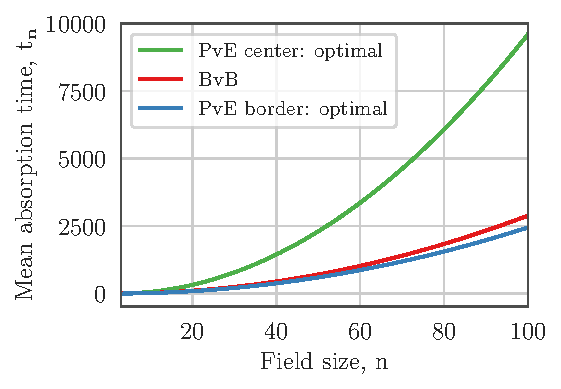
\includegraphics[width=\columnwidth,keepaspectratio,clip]{fig2.pdf}
    \caption{
        Квадратичные зависимости среднего времени поглощения от размеров поля для случаев: центр PvE для игрока A 
        (цель игрока оставаться внутри как можно дольше) -- зеленая линия, 
        граница PvE для игрока B (цель игрока достичь границу как можно скорее) -- синяя линия, 
        BvB (времена поглощения чистого случайного блуждания) -- красная линия.
    }  
    \label{fig:quadratic:time}
    \end{center}
\end{figure}


\subsection{Сравнение с экспериментальными результатами}\label{subsec:ch3/sec1/sub4}

Следующим шагом в анализе игровой динамики является рассмотрение сравнения результатов моделирования с результатами 
собранных игр в полевом эксперименте. Сбор траекторий в эксперименте осуществлялся с применением разработанной игры Random Walk Game
и участием нескольких десятков людей. Подробное описание эксперимента приведено в разделе \cref{subsec:ch2/sec2} <<Полевой эксперимент>>. Суммарно в режиме 
PvE было собрано $1062$ игры: $528$ -- игры за центр, $534$ -- игры за границу. 

Участники, цель которых была удерживать фишку как можно
дольше внутри поля в среднем показали $145.45$ ходов за игру. Сравнивая этот результат с предположительно оптимальной стратегией 
среднее время которой равно $\boldsymbol{\mathsf{t_{17}^{PvE A}}} = (17-2)^2 = 225$, получаем отставание на $54\%$ реальных игр от результатов моделирования.
Хотя игроки показали не оптимальное время игры, выбранная ими стратегия позволяет улучшить в $2$ раза результат относительно $75.2$ хода
в случае равновероятного выбора (BvB). Эксперимент показал, что рассматриваемая группа игроков способна распознать свойства игры 
и значительно улучшить среднее время игры несмотря на отсутствие априорного знания об оптимальной стратегии. 
В качестве подтверждения качества стратегии, найденной игроками, были получены относительные частоты для каждой позиции на поле
и проведено моделирование столкновения стратегий случайного выбора против стратегии игроков. В результате моделирования было получено 
характерное среднее время игры $145.85$ согласующееся со средним временем экспериментальных траекторий.

Результаты игр участников в случае PvE с целью скорейшего достижения границы продемонстрировали среднее количество ходов равное $71.12$.
В сравнении с предполагаемой оптимальной стратегией, среднее время которой равно $\boldsymbol{\mathsf{t_n^{PvE B}}} = \frac{(17-1)^2}{4} = 64$, игроки 
отстают на 7 ходов. Несмотря на такое отставание, среднее время игры у участников меньше на 4 хода, чем в случае равновероятного выбора. 
Аналогично предыдущему случаю игры за центр, игроки показали улучшение относительно случайного блуждания BvB и достаточно большой разрыв со средним временем игры
для предполагаемой оптимальной стратегии. Моделирование игровой динамики за счет столкновения стратегий равновероятного случайного выбора и 
частот выборов, полученных из эксперимента, продемонстрировало отличие среднего времени игры, равного $73.79$, относительно среднего числа ходов в траекториях игроков.
Предположительно, данное отличие вызвано неточными частотами в редко посещаемых состояниях. 

Результаты эксперимента корректно воспроизводятся при использовании частот из экспериментальных игр для случая PvE в
качестве входных вероятностей для процесса моделирования с применением эволюции вероятности и численного моделирования отдельных траекторий. 
Таким образом, частоты выбора соответствующих стратегий, определенные для каждого состояния, позволили нам интерпретировать множество $f_{ij}$ как усредненную стратегию, 
найденную группой участников эксперимента. Значения среднего времени игры представлены в сводной таблице (см. Таблицу~\cref{tab:time}).

\begin{table}[]
    %\setlength\extrarowheight{3pt}
    \fontsize{10pt}{10pt}\selectfont
    \begin{tabular}{|l|c|c|c|c|c|}%{|p{1.7cm}|C{1.2cm}|C{1.2cm}|C{1.2cm}|C{1.2cm}|C{1.2cm}|}
        
        \toprule
        %\multicolumn{1}{|c|}{\begin{tabular}[c]{@{}c@{}}Размер поля\\$17 \times 17$\end{tabular}} & \textbf{\begin{tabular}[c]{@{}c@{}}Random\\walk\end{tabular}} & \textbf{\begin{tabular}[c]{@{}c@{}}PvE центр\end{tabular}} & \textbf{\begin{tabular}[c]{@{}c@{}}PvE граница\end{tabular}} & \textbf{PvP} & \textbf{\begin{tabular}[c]{@{}c@{}}PvP\\ 400+\end{tabular}} \\ \hline
        Размер поля $17 \times 17$ & \textbf{BvB} & \textbf{PvE центр} & \textbf{PvE граница} & \textbf{PvP} & \textbf{PvP $400+$} \\ 
        \midrule
        \textbf{Количество игр} & -     & 528    & 534   & 500    & 13     \\ 
        %\specialrule{.1em}{.0em}{.0em}
        \midrule
        \textbf{Эксперимент}  & -     & 145.45 & 71.12 & 120.60 & 594.27 \\ 
        \textbf{Моделирование траекторий}  & 75.22 & 145.77 & 73.66 & 115.93 & 132.91 \\
        \textbf{Теория Марковских цепей}  & 75.21 & 145.85 & 73.79 & 116.22 & 133.22 \\
        \textbf{Эволюция вероятности}   & 75.21 & 145.85 & 73.79 & 116.22 & 133.22 \\ 
        \textbf{Оптимальная стратегия*}     & -     & 225.00 & 64.00 & -    & -      \\ 
        \bottomrule
    \end{tabular}
    \caption{
        Средние времена поглощения, полученные с применением различных подходов для 4 случаев игры: 
        BvB -- чистое случайное блуждание на квадратной решетке с поглощением на границе,
        PvE -- случай игры против стратегии равновероятного выбора с двумя целями: центр -- цель оставаться как можно дольше внутри поля, 
        граница -- цель как можно скорее достичь границы, случай PvP -- игры двух игроков с произвольными стратегиями,
        случай PvP 400+ -- игры двух игроков, имеющие количество ходов свыше 400.
        Значения представлены для поля размером $17 \times 17$. При моделировании траекторий использовалось $10^5$ запусков для сбора статистики.
        Моделирование эволюции вероятности происходило в течение первых $10^4$ шагов. 
        Моделирование траекторий, теория поглощающих Марковских цепей и эволюция вероятности были выполнены на основе частот,
        полученных в реальных играх в полевом эксперименте. Для случая BvB частоты стратегий игроков выбирались по 0.5 (равновероятный выбор одной из кнопок).
    }
    \label{tab:time}
\end{table}

Среднее время игр участников друг с другом (PvP) находится между средними временами поглощения для случаев PvE при игре за центр и при игре за границу. 
Среднее количество ходов в PvP-играх на 57 ходов больше, 
чем среднее время игры в предполагаемой оптимальной стратегии PvE с пограничной целью. 
Сравнение с режимом PvE за центр показывает на 25 ходов меньше среднее время игры в PvP по сравнению 
с экспериментальными играми PvE и примерно в 2 раза меньше в PvP по сравнению с предполагаемой оптимальной стратегией при игре за центр в случае PvE.

Среднее время поглощения, полученное путем моделирования для конкретных частот, 
совпадает со средним значением теории AMC (абсолютная ошибка составила менее $10^{-9}$). 
Таким образом, оба метода могут применяться для точного вычисления среднего времени поглощения для произвольных стратегий. 
Подход к моделированию траекторий $10^5$ показывает точность до целой части значения среднего времени игры.

\section{Четность времени игры}\label{sec:ch3/sec2}

Моделирование игрового процесса позволило идентифицировать различия между четной и нечетной продолжительностью игры. 
Для анализа четности вычислим вероятность закончить игру при четном и нечетном количестве ходов.
Результаты представлены в Таблице~\cref{tab:parity}. Экспериментальные результаты в PvE за границу показывают почти равные частоты окончаний на четных и нечетных ходах. 
Однако в случае игр за центр вероятность закончить на нечетном ходу в $2$ раза выше, чем на четном. Аналогичное поведение было обнаружено в режиме PvP. 
Эти результаты указывают на склонность игроков к завершению игры в нечетных состояниях (то есть состояний в которых нечетная сумма координат). 
Хотя нечетные поглощающие состояния наблюдаются чаще, примерно $30\%$ игр заканчиваются четными состояниями. 
Это, в свою очередь, показывает необходимость наличия ненулевой вероятности как нечетных, так и четных окончаний в соответствующих играх между двумя игроками.

В отличие от игры двух игроков, оптимальные стратегии для режимов PvE демонстрируют явное предпочтение четным концовкам в случае игры за границу и 
нечетным концовкам в случае игры за центр. Первый раз граничные состояния поля могут быть достигнуты за $8$ ходов или $\frac{n-1}{2}$ для произвольного размера поля, 
что соответствует четным количествам ходов ($n$ -- нечетное). Вероятность такого события для оптимальной стратегии равна $0.00815$ на поле размером $17 \times 17$. 
Возможность удерживать фишку внутри поля с вероятностью единица доступна только для первых $14$ ходов и на $15$-м ходу она будет поглощена с вероятностью 
приблизительно $0.000061$ в поле $17 \times 17$. В общем случае, поглощение произойдет с ненулевой вероятностью на нечетном $n-2$ ходу.

\begin{table}[]
    %\setlength\extrarowheight{3pt}
    \fontsize{10pt}{10pt}\selectfont
    \begin{tabular}{|l|c|c|c|c|c|}%{|p{1.7cm}|C{1.2cm}|C{1.2cm}|C{1.2cm}|C{1.2cm}|C{1.2cm}|}
        \toprule
        %\multicolumn{1}{|c|}{\begin{tabular}[c]{@{}c@{}}Размер поля\\$17 \times 17$\end{tabular}} & \textbf{\begin{tabular}[c]{@{}c@{}}Random\\walk\end{tabular}} & \textbf{\begin{tabular}[c]{@{}c@{}}PvE центр\end{tabular}} & \textbf{\begin{tabular}[c]{@{}c@{}}PvE граница\end{tabular}} & \textbf{PvP} & \textbf{\begin{tabular}[c]{@{}c@{}}PvP\\ 400+\end{tabular}} \\ \hline
        Размер поля $17 \times 17$ & \textbf{BvB} & \textbf{PvE центр} & \textbf{PvE граница} & \textbf{PvP} & \textbf{PvP $400+$} \\
        \midrule
        \textbf{Эксперимент} & --     & 30:70 & 51:49 & 35:65 & 15:84 \\
        \textbf{Моделирование траекторий} & 50:50 & 30:70 & 51:49 & 36:64 & 31:69 \\
        \textbf{Эволюция вероятности}  & 50:50 & 30:70 & 51:49 & 36:64 & 31:69 \\
        \textbf{Оптимальная стратегия*}    & --     & 0:100 & 100:0 & --   & --     \\
        \bottomrule
    \end{tabular}
    \caption{
        Отношение шансов закончить игру при четном числе ходов к нечетному (четное~$:$~нечетное). 
        Значения были получены разными подходами для 4 случаев игры: 
        BvB -- чистое случайное блуждание по двумерной конечной решетке, 
        PvE -- случай игры против стратегии равновероятного выбора с двумя целями: центр -- цель оставаться как можно дольше внутри поля, 
        граница -- цель как можно скорее достичь границы, случай PvP -- игры двух игроков с произвольными стратегиями,
        случай PvP 400+ -- игры двух игроков, имеющие количество ходов свыше 400. Значения представлены для поля размером $17 \times 17$
        Значения представлены для поля размером $17 \times 17$. При моделировании траекторий использовалось $10^5$ запусков для сбора статистики.
        Моделирование эволюции вероятности происходило в течение первых $10^4$ шагов. 
        Моделирование траекторий, теория поглощающих Марковских цепей и эволюция вероятности были выполнены на основе частот,
        полученных в реальных играх в полевом эксперименте. Для случая BvB частоты стратегий игроков выбирались по $0.5$ (равновероятный выбор одной из кнопок).
    }
    \label{tab:parity}
\end{table}

\section{Распределение времен игры}\label{sec:ch3/sec3}

Моделирование эволюции вероятностей и траекторий позволили вычислить точные и приближенные вероятности завершения игры на $k$-ом ходе. 
Применение этих методов требует определения конкретной смешанной стратегии в зависимости от положения на игровом поле. 
Случай BvB чистого случайного блуждания определяет простую стратегию равновероятного выбора из двух доступных вариантов независимо от положения на игровом поле. 
Дополнительно к экспериментальным данным были проанализированы две предложенные стратегии предполагаемого оптимального случайного блуждания в режиме PvE. 
Помимо аналитических стратегий были получены экспериментальные частоты выбора стратегий в каждом состоянии. 
На основе этих стратегий было проведено моделирование эволюции вероятности по игровому полю во времени, 
а также моделирование индивидуальных траекторий с использованием различных стратегий ($10^5$ реализаций на каждый случай). 
В результате были получены распределения времен поглощения, представленные на Рис.~\cref{fig:distribution_time}.

\begin{figure*}[t]
    \begin{center}
    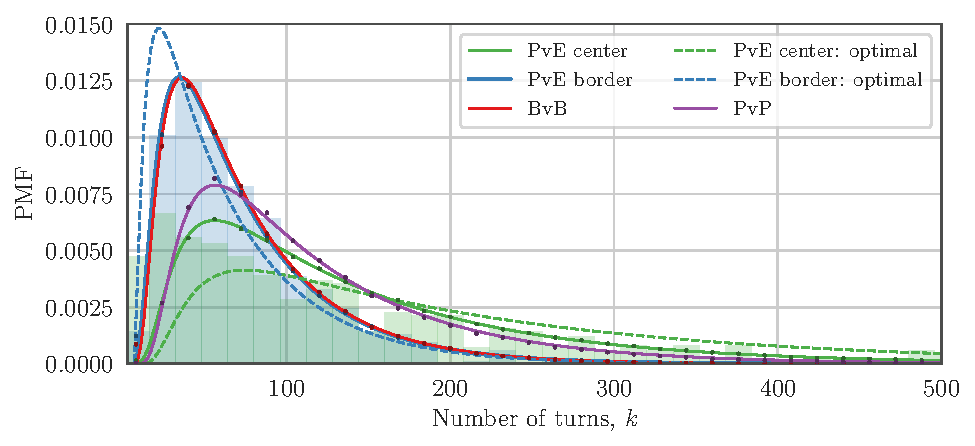
\includegraphics[width=\textwidth,keepaspectratio,clip]{fig3.pdf}
    \caption{
        Распределение количества ходов, полученное моделированием эволюции вероятности (сплошная линия) и численным моделированием (точки) 
        с использованием соответствующих стратегий игроков A и B. 
        Режим BvB (красная линия) представляет собой равновероятный выбор для обоих игроков. Кривые PvE (зеленый и синий) и PvP-режим (фиолетовая линия) 
        были построены на основе соответствующих усредненных стратегий по популяции. Противоположная стратегия в режиме PvE -- это стратегия равновероятного выбора. 
        Оптимальная стратегия для режима PvE в центре (зеленая пунктирная линия) -- держать фишку на диагональной лестнице. Оптимальная стратегия для режима границы PvE 
        (синяя пунктирная линия) -- выбирать движения только вдоль горизонтальной линии. Гистограммы, полученные экспериментально, представлены для режимов PvE 
        (зеленая и синяя области).
    }  
    \label{fig:distribution_time}
    \end{center}
\end{figure*}

При детальном рассмотрении у всех распределений наблюдаются различия в вероятностях на четных и нечетных ходах. 
Для оценки характерного поведения распределений, рассмотрим гистограмму с широкими бинами (длиной в $16$ ходов). 
Анализ показывает, что все режимы игры следуют одному и тому же паттерну:
\begin{itemize}
\item короткие партии встречаются редко;
\item распределение имеет одну моду с промежуточным числом ходов;
\item вероятность длинных игр экспоненциально уменьшается с увеличением длины игры.
\end{itemize}

Режим PvE за центр демонстрирует аналогичную форму распределения, за исключением того, что мода соответствует коротким играм, 
которая скрыта при отображении с выбранным размером бинов.

Хотя количество собранных траекторий в режиме PvP ($500$) не очень большое, в распределении наблюдались нехарактерно долгие игры с длиной более $400$ ходов. 
Вероятность получения таких игр согласно моделированию средней популяционной стратегии ниже $0.015$. 
Однако в играх участников было обнаружено $13$ длинных траекторий в диапазоне от $461$ до $964$ ходов со средним временем поглощения равным $594.27$. 
Обнаруженное отклонение можно объяснить «синхронизацией» между отдельными индивидуумами при длительном взаимодействии. 
Поскольку в среднем один ход занимает $4.5$ секунды, игра с $400$ ходами длится $30$ минут. 
Такое продолжительное время, в течение которого игрок B не может завершить игру, вызывает разочарование и снижает концентрацию, 
что может привести к бессознательному принятию решений, которые может легко предсказать игрок A. 
Потеря концентрации приводит к ухудшению способности человека производить выбор стратегий случайным образом. 
В связи с этим в игре могут возникать процессы «синхронизации».

Подробный анализ этих игр был выполнен путем отделения стратегий этих игр от основной части распределения. 
В результате моделирования столкновения противоположных стратегий для случая PvP 400+ было получено меньшее среднее время поглощения, составившее приблизительно $133.22$ ходов. 
Чтобы сравнить распределения таких игр, также было проведено моделирование эволюции вероятностей для частот, наблюдавшихся в стратегиях длительных игр. 
Соответствующие распределения, полученные для длинных игр, изображены на Рис.~\cref{fig:distribution_time_PvP}. Хотя распределение частот демонстрирует длинный хвост, 
лежащие в основе стратегии, которые появляются в «синхронизированных» играх, не воспроизводят появление столь же длинных игр. 
Таким образом, это демонстрирует наличие зависимости выбора игроков от скрытых факторов, которые нельзя объяснить только свойством цепи Маркова.


\begin{figure*}[t]
    \begin{center}
    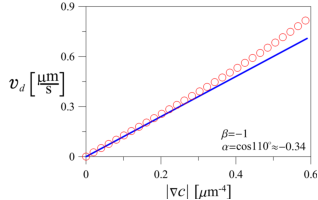
\includegraphics[width=\textwidth,keepaspectratio,clip]{fig4.pdf}
    \caption{
        Распределение времени поглощения для режима PvP (желтая гистограмма и фиолетовая линия) 
        по сравнению с моделированием частот направлений движения (зеленая линия) и частот стратегий (синяя линия), 
        наблюдаемых в длительных играх (более $400$ ходов). Частоты направлений движения для каждого состояния, полученные в 
        экспериментальных длинных играх, использовались для моделирования эволюции вероятностей найти фишку в узлах решетки. 
        Стратегии обоих игроков A и B в PvP с длиной ходов более $400$ использовались отдельно при моделировании.
    }  
    \label{fig:distribution_time_PvP}
    \end{center}
\end{figure*}


\section{Пространственное распределение}\label{sec:ch3/sec4}

Затем была проанализирована вероятность нахождения фишки в определенном состоянии во время игры. 
Как и в предыдущих разделах, проведено сравнение экспериментально полученных частот и результатов моделирования. 
Визуализации пространственных распределений для соответствующих стратегий изображены на Рис.~\cref{fig:distribution_states}.

\begin{figure}[t]
    \begin{center}
    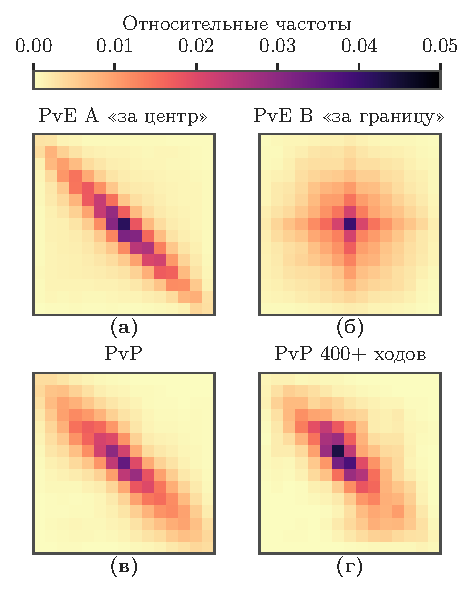
\includegraphics[width=\columnwidth,keepaspectratio,clip]{fig5.pdf}
    \caption{
        Двухмерные распределения частоты посещений узлов решетки, полученные в экспериментальных играх для 4 случаев: 
        PvE за центр, PvE за границу, игры двух игроков (PvP) и игры продолжительностью более $400$ ходов в режиме PvP.
    }  
    \label{fig:distribution_states}
    \end{center}
\end{figure}

Чистое случайное блуждание демонстрирует дискретное гауссово распределение в пространстве. 
Добавление игровой динамики в свою очередь меняет итоговую картину распределения. 
Как и следовало ожидать, режим PvE в играх за центр демонстрирует в основном движения по диагонали (см. Рис.~\cref{fig:distribution_states}A). 
Хотя это поведение совпадает с пространственным распределением в предложенной оптимальной стратегии, 
экспериментальные данные имеют больший разброс вокруг диагональных состояний, чем для оптимальной стратегии.

Оптимальная стратегия в случае игры PvE за границу демонстрирует вертикальные или горизонтальные линии состояний, 
по которым происходит перемещение фишки. В результате экспериментальных игр PvE за границу найдены 
3 основных паттерна в распределении (см. Рис.~\cref{fig:distribution_states}B): ожидаемые движения по прямым линиям, и 
отличное движение от оптимального паттерна -- это распределение, похожее на чистое случайное блуждание на двумерной квадратной решетке. 
Второй паттерн показывает попытку популяции найти более хорошую стратегию в двумерном пространстве, а не на одномерной линии. 
Однако уход одномерных отрезков увеличивает среднее время поглощения. Это объясняет небольшую разницу в средних временах 
поглощения между экспериментальным играми в случае PvE за границу и чистым случайным блужданием BvB.

Схема пространственного распределения в случае игры PvP (см. Рис.~\cref{fig:distribution_states}C) аналогична случаю PvE при игре за центр: 
фишка в основном движется по диагонали. Единственное отличие -- увеличенный разброс относительно диагональной линии, 
который показывает более сильную усредненную стратегию для игрока B, цель которого достичь границу, 
по сравнению с равновероятным случайным выбором (как в случае игры PvE за центр).
Дополнительной характерной особенностью случая PvP является более яркая выраженность
блужданий в левой верхней и правой нижней четвертях квадрата относительно центра, в сравнении со случаем PvE при игре за центр.
Посещение же двух других четвертей квадрата является более редким событием.

В заключение, было проанализировано пространственное распределение состояний в играх длиной более $400$ ходов. 
Вероятность расположения фишки в основном сосредоточена на главной диагонали, как и в предыдущих случаях (см. Рис.~\cref{fig:distribution_states}D). 
Тем не менее, распределение более компактно в центре поля и имеет более высокую вариацию вокруг главной диагонали 
по сравнению со случаями PvE за центр и PvP. Такое поведение предполагает более длительное нахождение фишки ближе к центру 
в длинных партиях с движением не только по диагонали, а также перпендикулярно ей.


\section{Анализ стратегий}\label{sec:ch3/sec5}

Далее, рассмотрим сравнение усредненных стратегий популяции для игроков A и B друг с другом, а также с оптимальными стратегиями. 
Для представления стратегий, визуализируем их в виде цветной двумерной матрицы с элементами, 
соответствующими состояниям на двумерной квадратной решетке (Рис.~\cref{fig:strategies}). 
Цвет элемента матрицы отображает частоту выбора первой кнопки из двух возможных вариантов в соответствии с правилами (см. Рис.~\cref{fig:controls}). 
Игрок А, старающийся сохранять фишку внутри поля, имеет два варианта: двигаться вверх/вправо или двигаться вниз/влево; 
игрок B старающийся как можно скорее достичь границы имеет также два выбора: двигаться вверх/вниз или двигаться влево/вправо. 
Разные цвета элементов матрицы демонстрируют, какой из двух выборов доминирует для каждого состояния в среднем по всем играм популяции.

\begin{figure*}[t]
    \begin{center}
    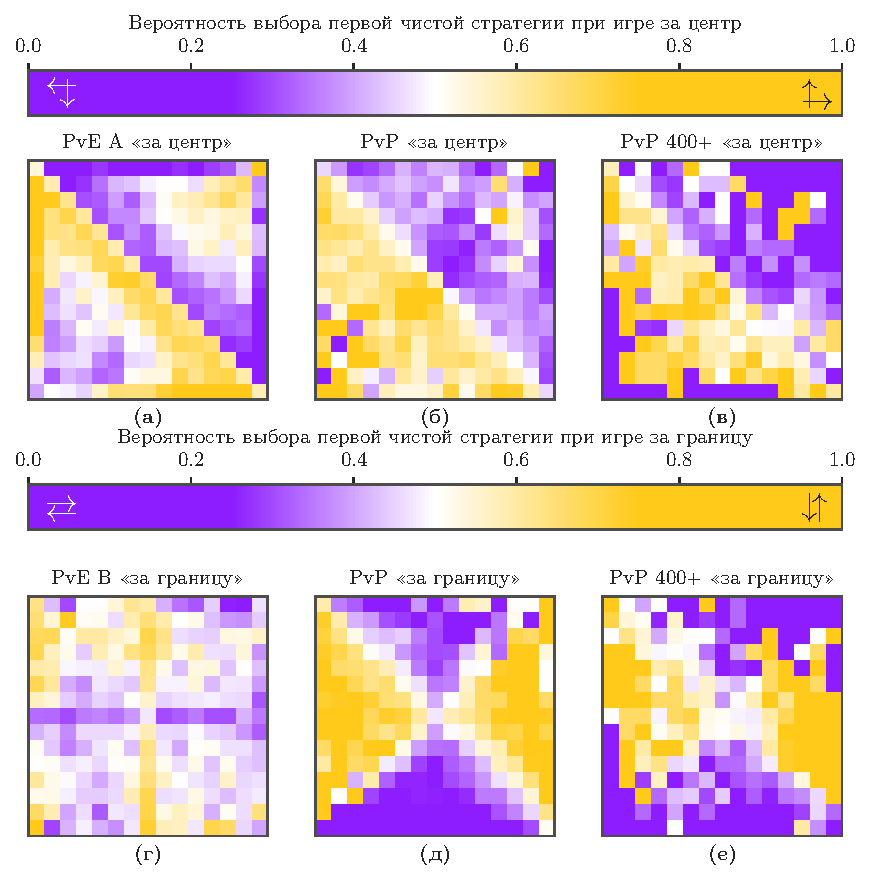
\includegraphics[width=\textwidth,keepaspectratio,clip]{fig6.pdf}
    \caption{
        Визуализация средних популяционных стратегий для разных режимов, полученных в эксперименте. 
        Цвет ячеек отображает частоту выбора первой чистой стратегии: для игры за центр (A, B, C) и для игры за границу (D, E, F).
    }  
    \label{fig:strategies}
    \end{center}
\end{figure*}

Стратегия, наблюдаемая в случае режима PvE за центр, демонстрирует в основном движение в направлении диагональных состояний (Рис.~\cref{fig:strategies}A). 
Однако состояния, удаленные от диагонали, показывают немного более высокие частоты противоположных стратегий. 
Обычно игроки выбирают уходить от границы, но в состояниях ближе к углам на боковой диагонали поведение становится более случайным 
(относительные частоты ближе к $0.5$). Экспериментальная стратегия на главной диагонали демонстрирует схожесть с первой предполагаемой оптимальной стратегией, 
рассмотренной в разделе \cref{subsec:ch3/sec1/sub3} <<Гипотеза об оптимальных стратегиях для случая PvE>>. Напротив, выбор игроков на границе отличается от второй предполагаемой оптимальной стратегии, 
которая предлагает всегда двигаться в направлении от границы. Это приводит к утечке вероятностей за пределы поля не только в углах главной диагонали, 
но и в других пограничных состояниях, что в свою очередь значительно снижает среднее время игры. 

Стратегия игрока играющего за центр в случае PvP аналогична стратегии PvE для игрока за центр (Рис.~\cref{fig:strategies}B). 
Более того, в среднем игроки предпочитают двигаться в направлении главной диагонали независимо от положения на решетке. 
Почти все состояния вблизи границы демонстрируют аналогичную стратегию, за исключением некоторых состояний с почти равной частотой обоих вариантов. 
По сравнению с режимом PvE за центр, игрок в случае PvP играющий за центр имеет немного меньшую уверенность в движении к главной диагонали 
(частоты ближе к $0.5$ в PvP по сравнению с PvE).

Стратегия PvE за границу четко определена на горизонтальной и вертикальной линиях (Рис.~\cref{fig:strategies}D). 
Хотя игроки чаще выбирают движение к ближайшей границе на центральных прямых, частоты в других состояниях не соответствуют общей схеме. 
В отличие от схожих стратегий PvE и PvP в случае игры за центр, стратегия PvP при игре за границу демонстрирует отличающееся поведение с четко прослеживаемым паттерном 
(Рис.~\cref{fig:strategies}E). 
В этом случае игроки действуют прямо противоположно режиму PvE за границу. Усредненная стратегия популяции предлагает выбирать движение 
по координатной линии имеющей наименьшее отклонение от центра. В результате плоскость решений разбивается на $4$ чередующихся треугольника. 
Хотя частоты близки к $0$ или $1$, имеется небольшая разница, которая свидетельствует о редких попытках движения к ближайшей границе.
Такое значительное отличие предположительно связано с очевидностью для игрока за центр выбора оппонента перемещаться в направлении границы.
Это заставляет игрока старающегося достичь границу реже делать попытки перемещения к границе для уменьшения шансов предсказать и противодействовать этому движению
со стороны второго игрока.

Для результирующих стратегий, полученных в длинных играх между двумя игроками (Рис.~\cref{fig:strategies}C,F), 
четких закономерностей не наблюдается из-за ограниченного количества игр. 
Однако наблюдается сходство принципов принятия решений с обычным случаем PvP.


\section{Выводы по главе 3}\label{sec:ch3/sec6}

В данной главе были рассмотрены основные результаты сравнения статистических свойств экспериментально
полученных траекторий и стратегий игроков с соответствующими результатами моделирования различными подходами. 
Предложена гипотеза об оптимальных средних временах достижения границы для двух случаев игры и 
рассмотрены соответствующие стратегии, достигающие оптимальных времен. Продемонстрирована оптимальность
данных стратегий и средних времен игры для случаев малого размера поля.
В главе для анализа игры Random Walk Game применены подходы численного моделирования, моделирования эволюции вероятности и полевого эксперимента,
на основе которых вычислены средние времена игры, распределения времен игры и пространственные распределения фишки на поле. 
Полученные результаты визуализированы с использованием языка Python 3.8 и библиотек numpy, scipy, matplotlib.

